\documentclass[10pt]{beamer}
\usefonttheme{professionalfonts,serif}
\def\newblock{\hskip .11em plus .33em minus .07em}
\usepackage[numbers,sort]{natbib}
\renewcommand{\rmdefault}{psbx}
\usepackage[utf8]{inputenc}
\usepackage[T1]{fontenc}
\usepackage{textcomp}
\usepackage{eulervm}

\usetheme{default}           % tips from David Blei
\useinnertheme{circles}
\useoutertheme{infolines}
\setbeamertemplate{headline}{}
\setbeamertemplate{navigation symbols}{}
\setbeamerfont{itemize/enumerate subbody}{size=\normalsize}
\setbeamerfont{itemize/enumerate subsubbody}{size=\normalsize}
\usecolortheme{seahorse}
\setbeamersize{text margin left=2mm,text margin right=2mm}

\graphicspath{{../../figures/}}

\definecolor{mypine}{rgb}{0.05,0.45,0.05}
\definecolor{mycyan}{rgb}{0.0,0.9,0.9}
\newcommand{\Red}{\textcolor{red}}
\newcommand{\Blue}{\textcolor{blue}}
\newcommand{\Green}{\textcolor{mypine}}
\newcommand{\PineGreen}{\textcolor{mypine}}
\newcommand{\Magenta}{\textcolor{magenta}}
\newcommand{\Cyan}{\textcolor{mycyan}}

\newcommand{\N}{\mathcal{N}}
\newcommand{\R}{\mathbb{R}}
\newcommand{\T}{{\scriptsize^{\top}}}
\newcommand{\D}{\mathcal{D}}
\newcommand{\F}{\mathcal{F}}
\newcommand{\E}{\mathbb{E}}
\newcommand{\V}{\mathbb{V}}
\newcommand{\M}{\mathcal{M}}
\newcommand{\KL}{\mathcal{KL}}
\newcommand{\cut}[1]{}
\newcommand{\trace}{\operatorname{trace}}

\newcommand{\bmu}{{\boldsymbol{\mu}}}
\newcommand{\btheta}{\boldsymbol{\theta}}
\newcommand{\bepsilon}{\boldsymbol{\epsilon}}
\newcommand{\balpha}{\boldsymbol{\alpha}}
\newcommand{\bbeta}{\boldsymbol{\beta}}
\newcommand{\bphi}{\boldsymbol{\phi}}
\newcommand{\bPhi}{\boldsymbol{\Phi}}
\newcommand{\bSigma}{\boldsymbol{\Sigma}}
\newcommand{\bpi}{\boldsymbol{\pi}}
\newcommand{\blambda}{\boldsymbol{\lambda}}

\newcommand{\argmax}{\operatorname{argmax}}
\newcommand{\argmin}{\operatorname{argmin}}
\newcommand{\ci}{{\bot\negthickspace\negthickspace\bot}} % conditional indep.
\newcommand{\neigh}{\operatorname{ne}}
\newcommand{\vectr}[2]{  \left[ \!\!\begin{array}{c} #1 \\
      #2 \end{array} \!\!\right]}
\newcommand{\deff}{\stackrel{\mathrm{def}}{=}}
\newcommand{\deldel}[2]{\frac{\partial #1}{\partial #2}}

\newcommand{\maketilde}{\raisebox{0.4ex}{\tiny $\sim$}}
\newcommand{\bfa}{\mathbf a}
\newcommand{\bfb}{\mathbf b}
\newcommand{\bfe}{\mathbf e}
\newcommand{\bff}{\mathbf f}
\newcommand{\bfk}{\mathbf k}
\newcommand{\bfm}{\mathbf m}
\newcommand{\bfn}{\mathbf n}
\newcommand{\bfp}{\mathbf{p}}
\newcommand{\bfs}{\mathbf s}
\newcommand{\bfu}{\mathbf u}
\newcommand{\bfx}{\mathbf x}
\newcommand{\bfy}{\mathbf y}
\newcommand{\bft}{\mathbf t}
\newcommand{\bfv}{\mathbf v}
\newcommand{\bfw}{\mathbf w}
\newcommand{\bfA}{\mathbf A}
\newcommand{\bfI}{\mathbf I}
\newcommand{\bfK}{\mathbf K}


\title{Gibbs Sampling}
\author{Carl Edward Rasmussen}
\date{October 28th, 2016}

\begin{document}


\begin{frame}
\titlepage
\end{frame}


\begin{frame}
\frametitle{Key concepts}

\begin{itemize}
\item bla
\end{itemize}

\end{frame}


\begin{frame}
\frametitle{How do we do integrals wrt an intractable posterior?}

Approximate \Blue{expectations} of a function $\phi(\bfx)$ wrt
\Blue{probability} $p(\bfx)$:
\[
\E_{p(x)}[\phi(x)]\;=\;\bar\phi\;=\;\int \phi(\bfx)\Red{p(\bfx)}d\bfx,
\text{\ \ where\ \ }\bfx\in\R^D,
\]
when these are not analytically tractable, and typically $D\gg1$.
\begin{center}
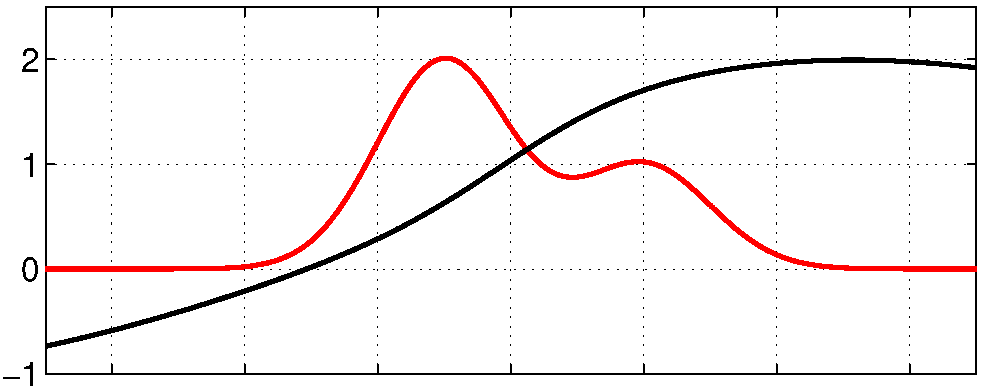
\includegraphics[width=0.7\textwidth]{mc0}
\end{center}
Assume that we can evaluate $\phi(x)$ and $\Red{p(x)}$.
\end{frame}


\begin{frame}
\frametitle{Numerical integration on a grid}

Approximate the integral by a sum of products
\[
\int \phi(\bfx)\Red{p(\bfx)}d\bfx\;\simeq\;\sum_{\tau=1}^T\phi(\bfx^{(\tau)})\Red{p(\bfx^{(\tau)})}\Delta\bfx,
\]
where the $\bfx^{(\tau)}$ lie on an equidistant grid (or fancier
versions of this).

\centerline{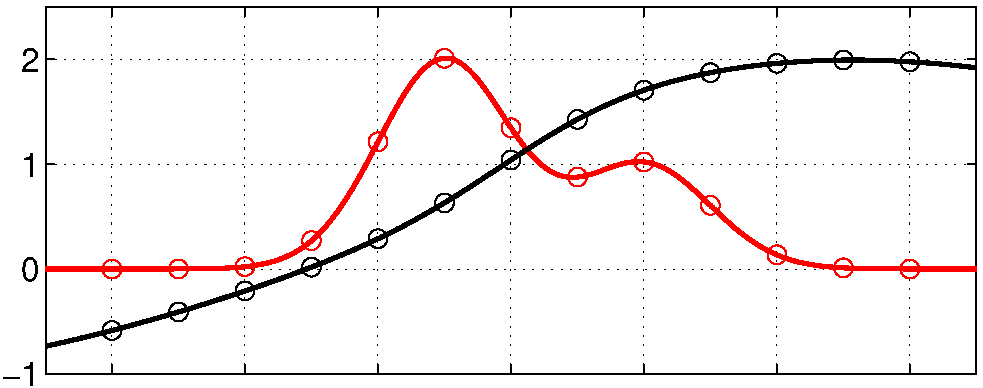
\includegraphics[width=0.7\textwidth]{mc1}}

\Blue{Problem:} the number of grid points required, $k^D$, grows
exponentially with the dimension $D$. Practicable only to $D=4$ or so.
\end{frame}


\begin{frame}
\frametitle{Monte Carlo}

The fundamental basis for Monte Carlo approximations is
\[
\E_{\Red{p(x)}}[\phi(\bfx)]\;\simeq\;\hat\phi\;=\;\frac{1}{T}\sum_{\tau=1}^T\phi(\bfx^{(\tau)}),
\text{\ \ where\ \ }\bfx^{(\tau)}\sim \Red{p(\bfx)}.
\]

\centerline{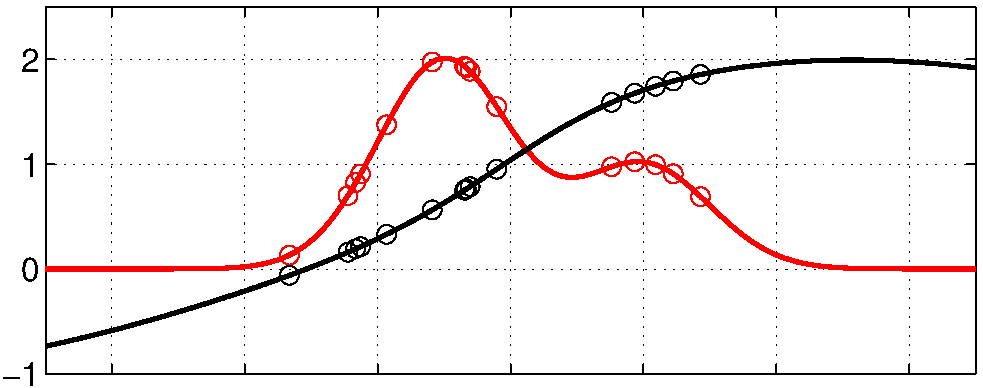
\includegraphics[width=0.7\textwidth]{mc4}}

Under mild conditions, $\hat\phi\rightarrow\E[\phi(\bfx)]$ as
$T\rightarrow\infty$. For moderate $T$, $\hat\phi$ may still be a good
approximation. In fact it is an \emph{unbiased} estimate with
\[
\V[\hat\phi]\;=\;\frac{\V[\phi]}{T}, \text{\ \ where\ \ }
\V[\phi]\;=\;\int \big(\phi(\bfx)-\bar\phi\big)^2\Red{p(\bfx)}d\bfx.
\]
\Blue{Note}, that this variance is \Blue{\emph{independent}} of the dimension
$D$ of $\bfx$.
\end{frame}


\begin{frame}
\frametitle{Markov Chain Monte Carlo}

This is great, but \Blue{how do we generate random samples} from
$\Red{p(\bfx)}$?

If $\Red{p(\bfx)}$ has a standard form, we may be
able to generate \Blue{\emph{independent}} samples.

\underline{Idea:} could we design a Markov Chain,
$\Blue{q(\bfx'|\bfx)}$, which generates (dependent) samples from the
desired distribution $\Red{p(\bfx)}$?
\[
\bfx \rightarrow \bfx' \rightarrow \bfx'' \rightarrow  \bfx'''
\rightarrow \ldots
\]


One such algorithm is called \Blue{\emph{Gibbs sampling}}: for each
component $i$ of $\bfx$ in turn, sample a new value from the
conditional distribution of $x_i$ given all other variables:
\[
x_i'\;\sim\;p(x_i|x_1,\ldots,x_{i-1},x_{i+1},\ldots,x_D).
\]
It can be shown, that this will eventually generate dependent samples from the 
joint distribution $\Red{p(\bfx)}$.

Gibbs sampling reduces the task of sampling from a joint distribution,
to sampling from a sequence of univariate conditional distributions.
\end{frame}


\begin{frame}
\frametitle{Gibbs sampling example: Multivariate Gaussian}

20 iterations of Gibbs sampling on a bivariate Gaussian; both
conditional distributions are Gaussian.

\begin{center}
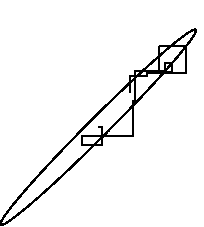
\includegraphics[width=0.4\textwidth]{bvg-gibbs}
\end{center}

Notice that \Blue{strong correlations} can \Blue{slow down} Gibbs sampling.
\end{frame}


\begin{frame}
\frametitle{Gibbs Sampling}

Gibbs sampling is a parameter free algorithm, applicable if we know
how to sample from the conditional distributions.

{\bf Main disadvantage:} depending on the target distribution, there may be
very strong correlations between consecutive samples.

To get less dependence, Gibbs sampling is often run for a long time,
and the samples are thinned by keeping only every 10th or 100th
sample.

It is often challenging to judge the \emph{effective correlation
  length} of a Gibbs sampler. Sometimes several Gibbs samplers are run
from different starting points, to compare results.
\end{frame}


\end{document}
